\section{Introduction}
\subsection{Breast Cancer}
\begin{frame}{Breast Cancer in Chile}
    \begin{columns}
        \begin{column}{0.6\textwidth}
            \begin{itemize}
                \item Worldwide, has an average mortality rate of \num{13.6} per \num{100000} women in 2020 \citef{BreastCancerStatistics}
                \item In Chile, has an average mortality rate of \num{11.8} per \num{100000} women, as of 2018 \citef{ministeriodesaludInformeVigilanciaCancer2021}
                \item Early screening is effective but dependant on multiple social, healthcare and economic factors.
                \item Early diagnosis and survival rate in Chile has increased due to the implementation of screening programs \citef{castilloResultadosTratamientoCancer2017}
            \end{itemize}
        \end{column}
        \begin{column}{0.4\textwidth}
            \begin{figure}
                \centering
                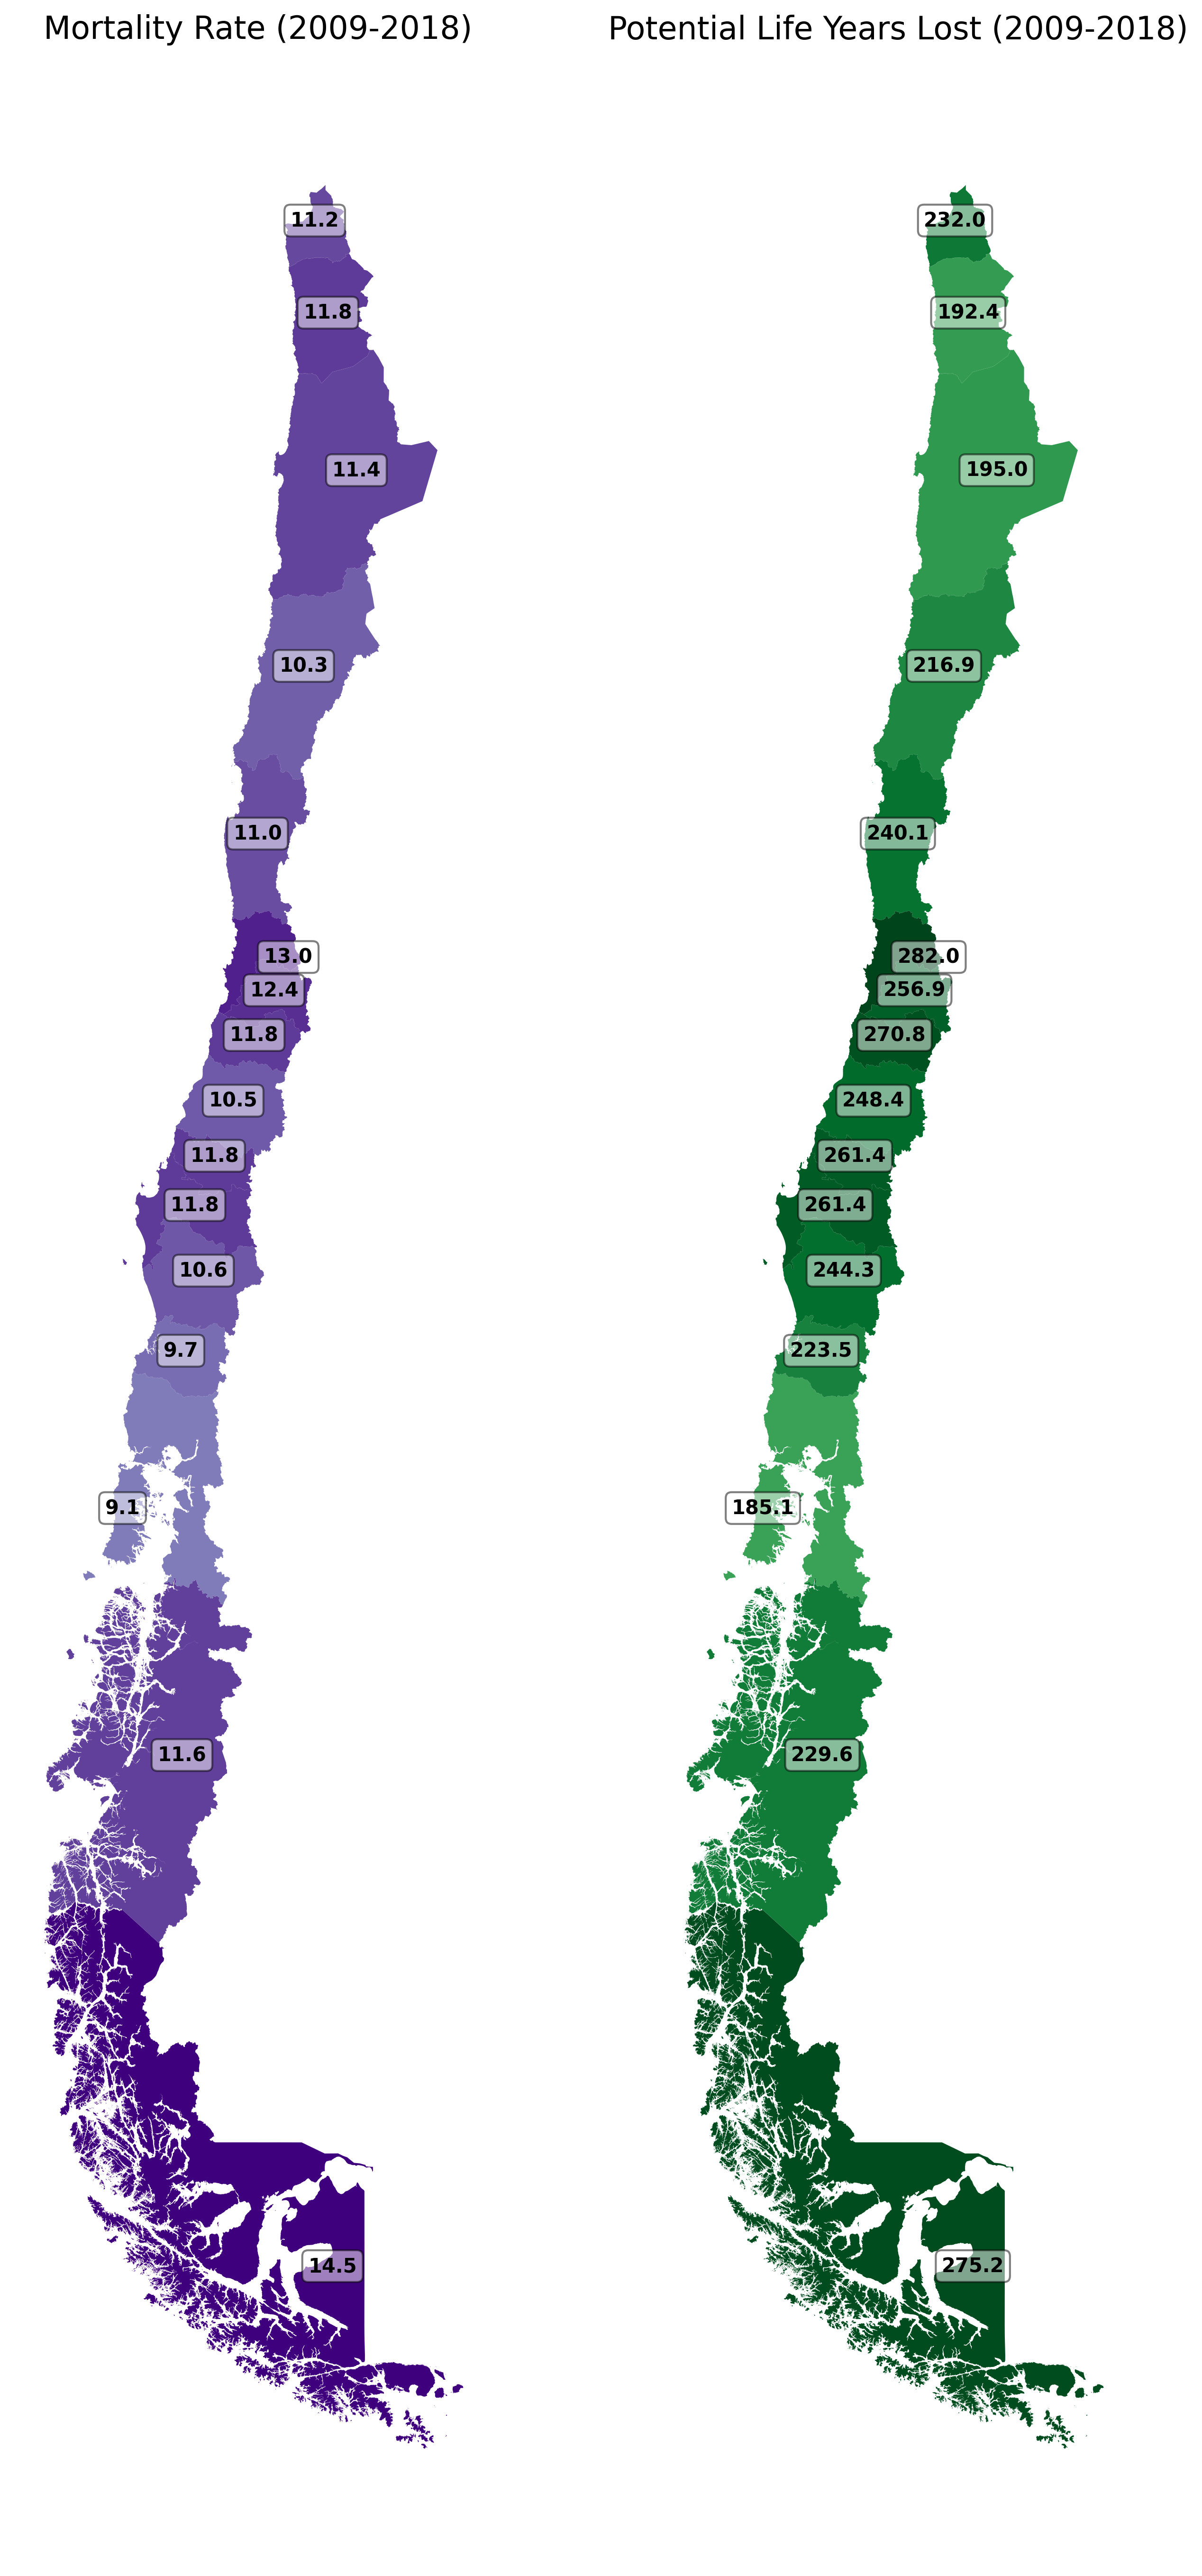
\includegraphics[height=0.5\textheight]{imagenes/mortalidad.png}
                \caption{Mortality rate and number of potential lost years of life due to breast cancer of Chilean Women per region (2009-2018)}
            \end{figure}
        \end{column}
    \end{columns}
        
\end{frame}

% Descripcion del cancer de mama
\begin{frame}{AI in breast Cancer}
    \begin{columns}
        \begin{column}{0.6\textwidth}
            \begin{itemize}
                \item Machine Learning and Deep Learning models have been implemented for the detection of breast cancer in mammograms. \citef{rodriguez-ruizDetectionBreastCancer2018}
                \item Current Challenges:
                \begin{itemize}
                    \item Detection of breast lesion location in mammograms \citef{diazSonSistemasInteligencia2021}
                    \item Visualisation tools for interpretation of prediction models.
                    \item Breast Density Estimation
                    \item Breast image classification beyond malignity.
                \end{itemize}
            \end{itemize}
        \end{column}
        \begin{column}{0.4\textwidth}
            \begin{figure}
                \centering
                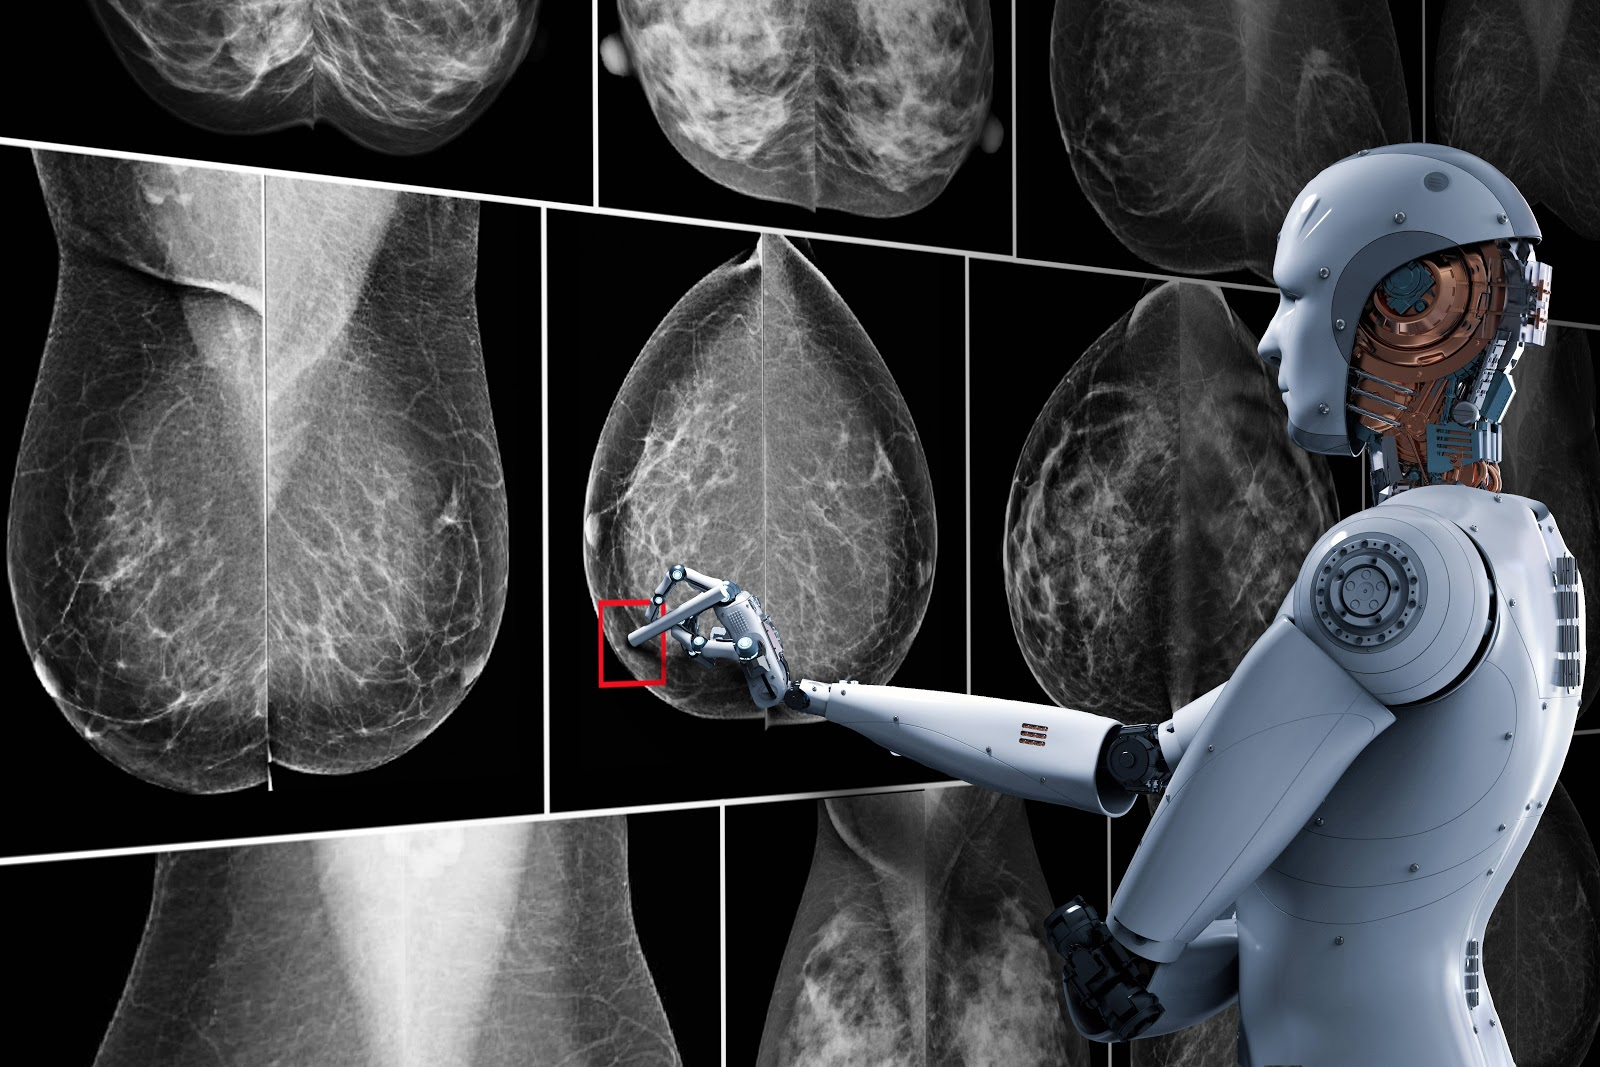
\includegraphics[width=\textwidth]{imagenes/nvidiaAI.jpg}
            \end{figure}
        \end{column}
    \end{columns}
    
\end{frame}

% metodos de localizar hallazgos
\begin{frame}{Pathological Findings Detection for Breast Cancer}
    \begin{columns}
        \begin{column}{0.3\textwidth}
            \citeauthor{ertosunProbabilisticVisualSearch2015} proposed a Deep Learning model for visual search in mammograms using a regional probabilistic approach. \citef{ertosunProbabilisticVisualSearch2015}

            \begin{figure}
                \centering
                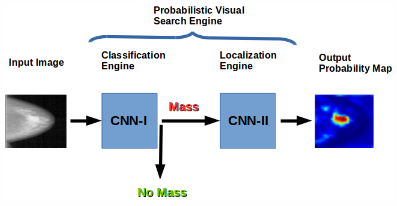
\includegraphics[width=\textwidth]{imagenes/ertosun_probmodel.png}
                \caption{Probabilistic Visual Search Engine proposed by \citeauthor{ertosunProbabilisticVisualSearch2015}}
            \end{figure}
        \end{column}
        \pause
        \begin{column}{0.3\textwidth}
            \citeauthor{frankDeepLearningArchitecture2023}
            proposed using YOLO V5 for detection of breast lesions, combined with EfficientNet for classification of masses and microcalcifications.
            \citef{frankDeepLearningArchitecture2023}

            \begin{figure}
                \centering
                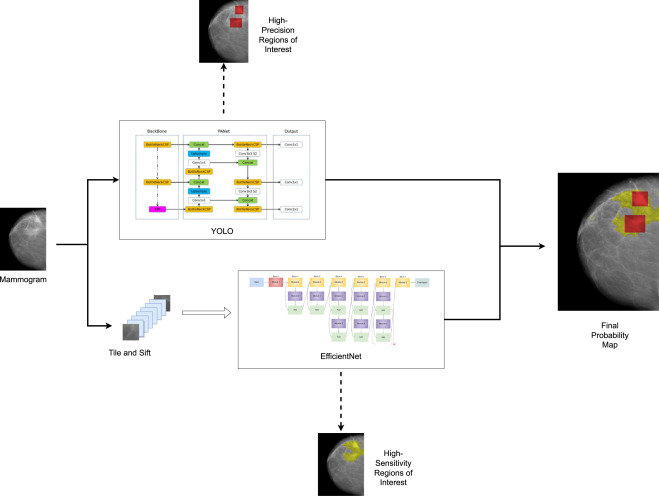
\includegraphics[height=0.3\textheight]{imagenes/frankyolo.jpg}
                \caption{Combined detection model and classifier for breast cancer proposed by \citeauthor{frankDeepLearningArchitecture2023}}
            \end{figure}
        \end{column}
        \pause
        \begin{column}{0.3\textwidth}
            \citeauthor{yiOptimizingVisualizingDeep2017} proposed a model for visualization of shared features between views of the breast for classification of benign and malignant breast tumours.
            \citef{yiOptimizingVisualizingDeep2017}
            \begin{figure}
                \centering
                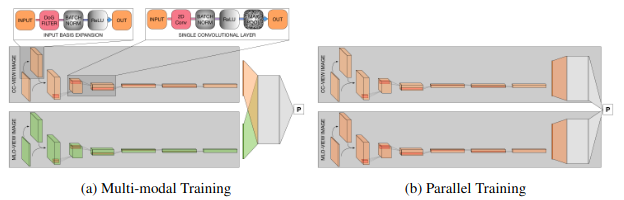
\includegraphics[width=\textwidth]{imagenes/yiparallel.png}
                \caption{Multimodal architecture proposed by \citeauthor{yiOptimizingVisualizingDeep2017} for visualization of shared features between views of the breast.}
            \end{figure}
        \end{column}
    \end{columns}
\end{frame}

% Propuesta del proyecto
\subsection{Proposal}
\begin{frame}{Our Proposal}
    Our study proposes a Deep Learning Classifier trained on cropped segments of mammograms for multi-label classification of pathological findings.

    General Inspection of the complete image using local patches to identify the probability of the presence of a pathological finding.

    \begin{figure}
        \centering
        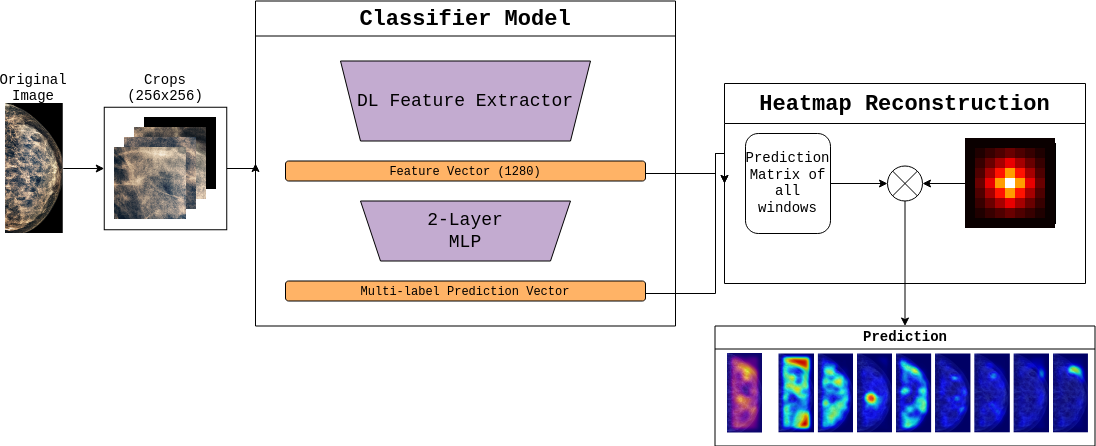
\includegraphics[height=0.5\textheight]{imagenes/modelo.png}
    \end{figure}
\end{frame}

